\documentclass[12pt, twoside]{article}
\usepackage[letterpaper, margin=1in, headsep=0.2in]{geometry}
\setlength{\headheight}{0.6in}
%\usepackage[english]{babel}
\usepackage[utf8]{inputenc}
\usepackage{microtype}
\usepackage{amsmath}
\usepackage{amssymb}
%\usepackage{amsfonts}
\usepackage{siunitx} %units in math. eg 20\milli\meter
\usepackage{yhmath} % for arcs, overparenth command
\usepackage{tikz} %graphics
\usetikzlibrary{quotes, angles}
\usepackage{graphicx} %consider setting \graphicspath{{images/}}
\usepackage{parskip} %no paragraph indent
\usepackage{enumitem}
\usepackage{multicol}
\usepackage{venndiagram}

\usepackage{fancyhdr}
\pagestyle{fancy}
\fancyhf{}
\renewcommand{\headrulewidth}{0pt} % disable the underline of the header
\raggedbottom
\hfuzz=2mm %suppresses overfull box warnings

\usepackage{hyperref}

\fancyhead[LE]{\thepage}
\fancyhead[RO]{\thepage \\ Name: \hspace{4cm} \,\\}
\fancyhead[LO]{BECA / Dr. Huson / Geometry\\*  Unit 11: Circle angles, sectors, arcs \\* 6 March 2023}

\begin{document}

\subsubsection*{11.6 Classwork: Data visualization with pie charts}
\begin{enumerate}
\item The \emph{pie chart} below shows the proportion of two subsets of a population, one represented in blue and one in orange. Dotted lines divide the circle in eight equal sectors for reference.
  \begin{multicols}{2}
  \raggedcolumns
  \begin{enumerate}[itemsep=1.5cm]
    \item Estimate the area of the blue sector as a fraction of the circle and as a decimal.
    \item The central angle of the orange sector measures $55^\circ$. Find the fraction of circle's area shaded orange as a fraction and a decimal.
  \end{enumerate}
  \begin{tikzpicture}[scale=0.8]
    \filldraw [color=blue, fill=blue!20, thick]
    (0,0)--(0:4) arc (0:135:4)--(0,0);
    \draw (0,0) circle[radius=4];
    %\draw [thick] (0:4) arc (0:36:4);
    %\draw [thick]
    %(0:4) node[right] {$A$}--
    %(0,0) node[below left] {$O$}--
    %(36:4) node[right] {$B$};
    \draw [thick, dotted](45:4)--(0,0)--(90:4);
    \draw [thick, dotted](135:4)--(0,0)--(180:4);
    \draw [thick, dotted](0:4)--(0,0)--(-135:4);
    \draw [thick, dotted](-45:4)--(0,0)--(-90:4);
    \filldraw [color=orange, fill=orange!20, thick]
    (0,0)--(-10:4) arc (-10:-65:4)--(0,0);
    \draw [thick, <->] (-10:1) arc (-10:-65:1);
    \node at (-35:1.5) {$55^\circ$};
  \end{tikzpicture}
  \end{multicols}

\item We use circle sectors (pie charts) to communicate. This map shows the most important of the 3991 coronavirus variants as they evolve across the world.
\begin{enumerate}[itemsep=0.7cm]
  \item In Europe, estimate the proportion of covid-19 identified as B.1.1.7 (light blue).
  \item In South America, which is more prevalent B.1.1.7 or P.1 (light orange)?
  \item In North America, what proportion of samples remain ``unassigned'' (gray)?
\end{enumerate}
  \begin{center}
    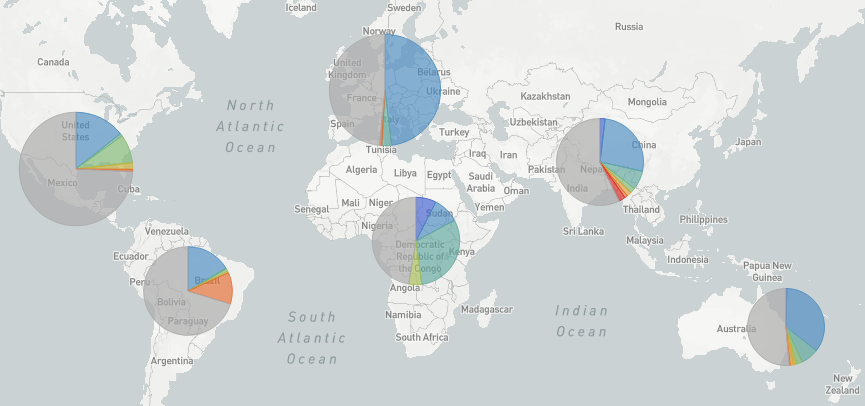
\includegraphics[width=18cm]{../graphics/11Covid_map.png}
  \end{center}
  \begin{flushright}
    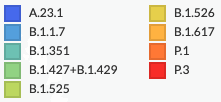
\includegraphics[width=5cm]{../graphics/11Covid_map_legend.png}
  \end{flushright}
  %https://nextstrain.org/ncov/global?c=emerging_lineage&dmin=2020-12-21&p=full&r=region



\item Ten values from one to five are displayed as a dot plot below on the right. \\[0.5cm]
The data is to be represented as a \emph{pie chart}. The red sector has been drawn to represent data with value equalling five. (Dotted lines divide the circle in ten equal sectors for reference.)
  \begin{multicols}{2}
  \begin{tikzpicture}[scale=0.8]
    \filldraw [color=blue, fill=blue!20, thick]
    (0,0)--(0:4) arc (0:30:4);
    \draw (0,0) circle[radius=4];
    \draw [thick, dashed, ->] (30:4) arc (30:45:4);
    \draw [color=blue, dashed, thick, ->] (0:2) arc (0:50:2);
    %\draw [thick]
    %(0:4) node[right] {$A$}--
    %(0,0) node[below left] {$O$}--
    %(36:4) node[right] {$B$};
    \draw [thick, dotted](72:4)--(0,0)--(108:4);
    \draw [thick, dotted](144:4)--(0,0)--(180:4);
    \draw [thick, dotted](-72:4)--(0,0)--(-108:4);
    \draw [thick, dotted](0:4)--(0,0)--(-144:4);
    \filldraw [color=red, fill=red!20, thick]
    (0,0)--(0:4) arc (0:-72:4)--(0,0);
    \node at (-35:2.5) {$5$};
    \node [color=blue] at (35:3) {$1$};
  \end{tikzpicture}
  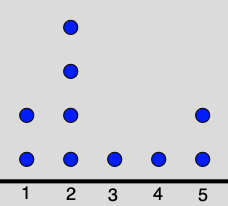
\includegraphics[width=5cm]{../graphics/11DotPlot.png}
  \end{multicols}
  \begin{enumerate}
    \item Shade the appropriate portion of the pie chart in blue to represent the data with value equalling one.
    \item Complete the rest of the pie chart using other colors to mark sectors for the data equalling two, three, and four.
  \end{enumerate}


\end{enumerate}
\end{document}